\documentclass[aspectratio=169,notheorems,8pt]{beamer}

\usepackage{algorithm}
\usepackage{algpseudocode}
\usepackage{alltt}
\usepackage{amsfonts}
\usepackage{amsmath}
\usepackage{amssymb}
\usepackage{bm}
\usepackage{booktabs}
\usepackage{graphicx}
\usepackage{mathrsfs}
\usepackage{mleftright}
\usepackage{parskip}
\usepackage{physics}
\usepackage{tikz}

\usetikzlibrary{arrows.meta, positioning}

\newcommand{\E}{\mathbb{E}}
\newcommand{\N}{\mathbb{N}}
\newcommand{\R}{\mathbb{R}}
\newcommand{\Z}{\mathbb{Z}}
\newcommand{\dom}{\mathrm{dom}}
\newcommand{\im}{\mathrm{im}}
\newcommand{\concat}{\mathbin{\|}}
\newcommand{\setmid}{\;\middle|\;}

\title{Vision World Models for Competitive Snake Playing}
\author{Team 5}
\date{March 2026}

\begin{document}

\maketitle

\section{Problem}

\begin{frame}
It is sometimes claimed that we are close to having AI with ``superintelligence''.
\begin{figure}
	\centering
	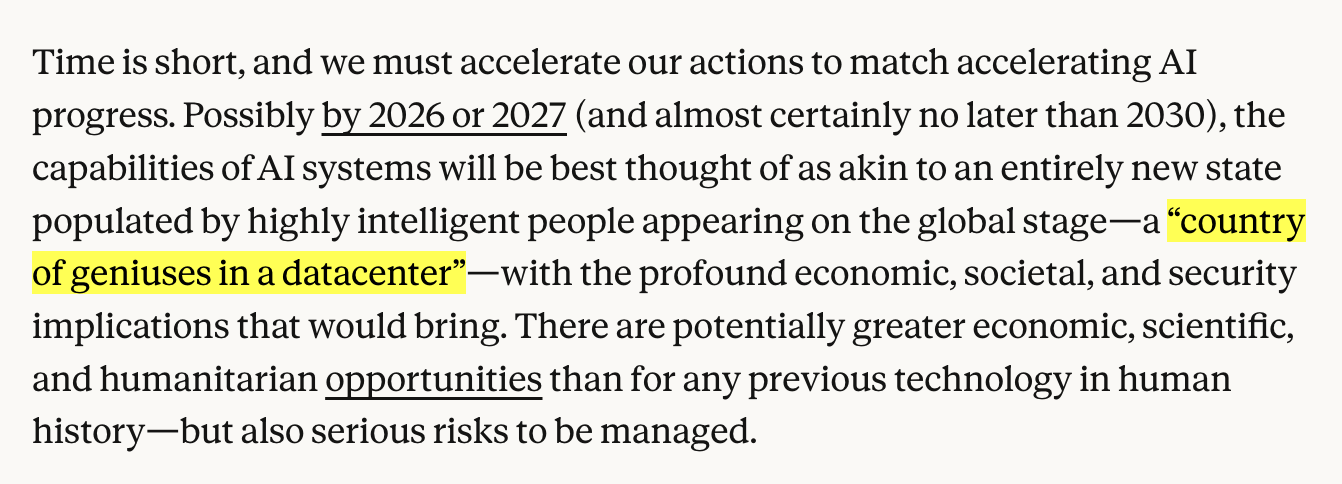
\includegraphics[width=0.5\textwidth]{anthropic-claim.png}
\end{figure}
Arguably, we barely have any AI with ``human-level intelligence''.
For example:
\begin{itemize}
	\item A 10 year old can often learn to fill up a dishwasher within \textbf{minutes}.
	\item A 17 year old can often learn to drive a car within \textbf{tens of hours}.
	\item Yet we (still) do not have level 5 ``fully-autonomous'' self-driving cars with \textbf{millions of hours} of training data.
\end{itemize}
\end{frame}

\begin{frame}
How might machines learn like animals?

(L)LMs are popular now, but limited by construction.
Consider the standard transformer (Vaswani et al., 2017):
\begin{itemize}
	\item It does a fixed amount of computation per token at inference.
	\item It does not model the consequences of its actions at inference.
	\item If it is autoregressive with a non-zero probability $\varepsilon\in\R_{[0,1]}$ of error (by generating a "bad" token) at each generation step, and errors are independent across steps, then the probability of generating an error-free token sequence decreases exponentially with sequence length $n\in\N$ because:
	$$
		(1-\varepsilon)^{n}\approx\exp(-\varepsilon n)
	$$
	\item The real world often has nothing to do with language (Einstein, 1931); humans use discrete, low-bandwidth, and clear symbols for effective communication, but the real world is often continuous, high-bandwidth, and noisy (LeCun, 2025).
\end{itemize}
\end{frame}

\begin{frame}
World models have been proposed as an approach to human-level AI.

Multiplayer Snake has been put forward as a research request by OpenAI.
\begin{figure}
	\centering
	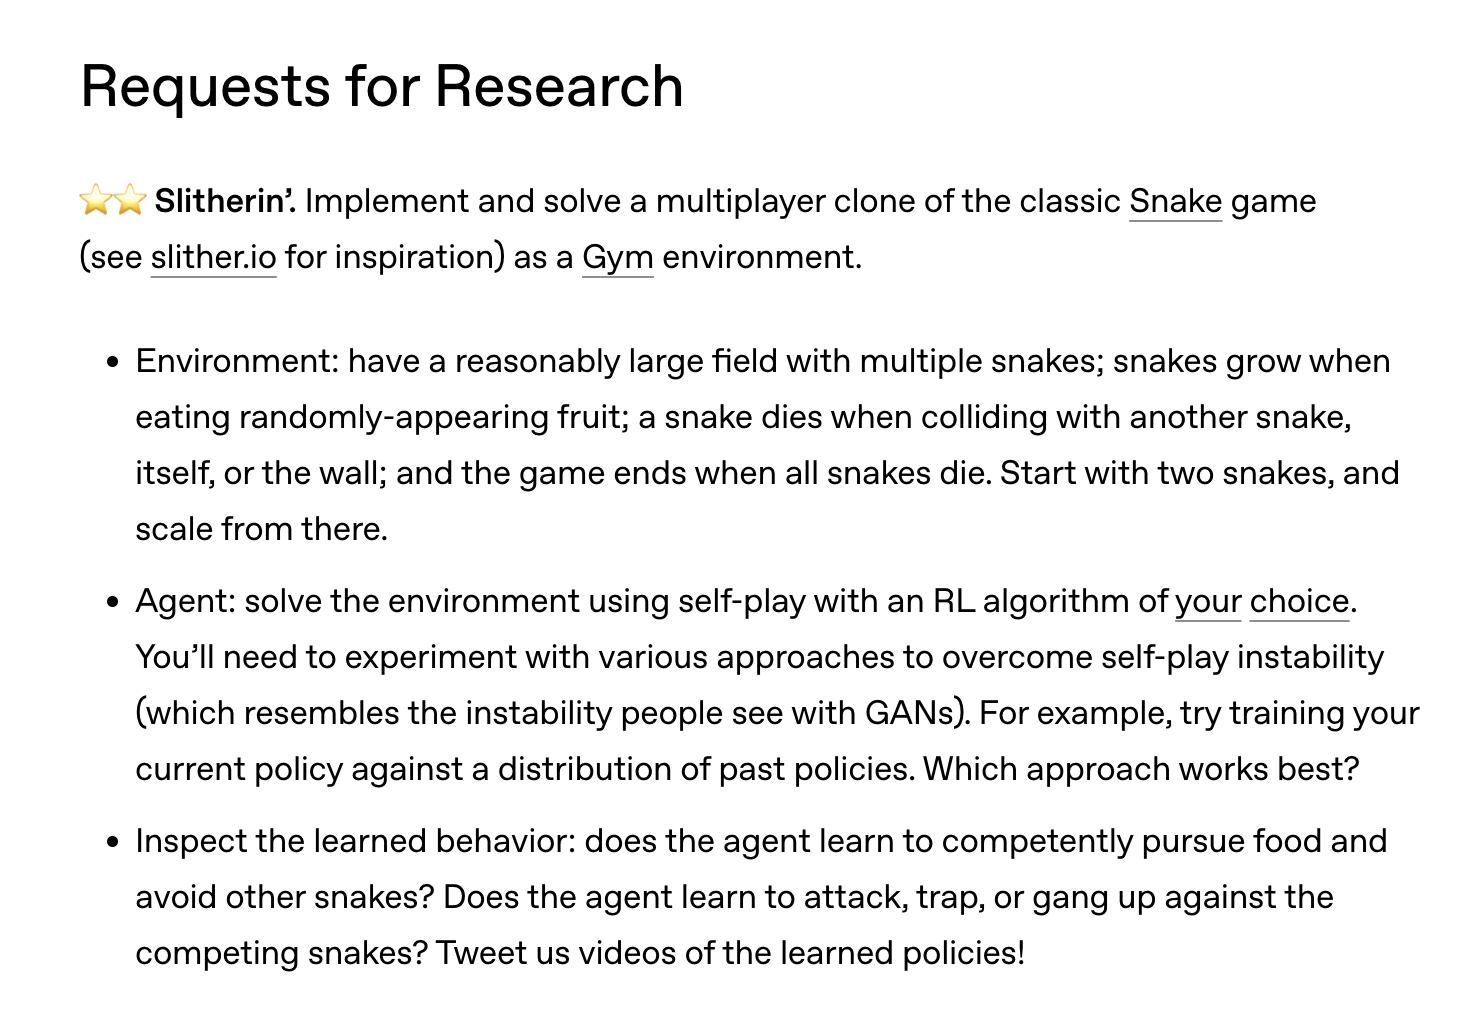
\includegraphics[width=0.5\textwidth]{openai-request.png}
\end{figure}
As our research contribution, we investigate vision world models in the simple setting of competitive Snake.
\end{frame}

\section{Proposal}

\begin{frame}[fragile]{Data}
We can simulate the game to collect (image, action, next image, cost) tuples in a dataset:
\begin{alltt}
initialise snakes
initialise food
initialise time
initialise dataset

while a snake is alive:
	translate each snake
	grow any snake on food

	mark as dead each snake whose head is on a wall or body
	for each cell with multiple heads:
		mark as dead each snake but random one from longest ones in cell
	remove each snake marked as dead

	respawn food if eaten
	add to dataset (image, action, next image, cost)
	increment time
\end{alltt}
\end{frame}

\begin{frame}{Data}
	\begin{table}[H]
		\centering
		\begin{tabular}{ll}
			cell & colour \\
			\midrule
			background & black \\
			body of playable snake & blue \\
			head of playable snake & ceil(mean(blue, white)) \\
			body of non-playable snake & red \\
			head of non-playable snake & ceil(mean(red, white)) \\
			food & green \\
		\end{tabular}
	\end{table}
	\begin{figure}
		\centering
		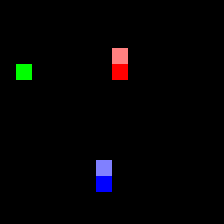
\includegraphics[width=0.2\textwidth]{snake-grid.png}
	\end{figure}
	We can colour and render the grid at arbitrary size using rasterisation.
\end{frame}

\begin{frame}{Data}
We can numerically encode the preference of ``avoiding death beats pursuing growth''.

For example, the cost at time $t\in\N$ can be a numerically encoded preference
$$
	c_{t}
	=
	\mleft(1+\mleft\lceil\frac{1}{1-\gamma}\mright\rceil\mright)
	d_{t}
	-
	g_{t}
$$
where $\gamma\in\R_{[0,1]}$ is a discount factor,
and $d_{t}$ is $1$ if death occurred at time $t+1$ (and $0$ otherwise),
and $g_{t}$ is $1$ if growth occurred at time $t+1$ (and $0$ otherwise).\footnote{The coefficient derives from the series $\sum_{t=0}^{\infty}\gamma^{t}=\frac{1}{1-\gamma}$.}
\end{frame}

\begin{frame}{Data (for rigour)}
Let $\mathrm{L}\in\N_{\geq 1}$ be a grid extent,
and $\mathrm{U}\in\N_{\geq 1}$ be an upsampling factor,
and $\mathrm{S}\in\N_{\geq 1}$ be a number of snakes.
\begin{align*}
	\mathcal{G}
	&=
	[1..\mathrm{L}]^{2}
	\tag{grid}
	\\
	\mathcal{A}
	&=
	\{(0,0),(0,1),(0,-1),(-1,0),(1,0)\}
	\tag{action space}
	\\
	\mathcal{M}
	&=
	\mathcal{A}\setminus\{(0,0)\}
	\tag{movement space}
	\\
	\mathcal{S}
	&=
	\bigcup_{n\geq 2}\mleft\{
		\bm{s}\in(\Z\times\Z)^{n}
		\setmid
		\forall i\in[1..n-1]\mleft(
			s_{i+1}-s_{i}\in\mathcal{M}
		\mright)
	\mright\}
	\tag{snake space}
	\\
	\mathcal{F}
	&=
	\mathcal{G}\cup\{\perp\}
	\tag{food space}
	\\
	\delta
	&:
	\mathcal{S}\times\N\to\mathcal{A}
	\tag{action oracle}
	\\
	\mathcal{O}(\bm{S})
	&=
	\mleft\{
		s_{i}
		\mid
		\bm{s}\in\bm{S}
		\land
		i\in[1..\abs{\bm{s}}]
	\mright\}
	\tag{snake occupancy}
	\\
	\rho
	&:
	\mathcal{G}^{2\mathrm{S}}
	\to
	(\mathcal{G}\times\mathcal{G})^{\mathrm{S}}
	\\
	\rho(\bm{x})
	&=
	(
		(x_{2i-1},x_{2i})
	)_{i=1}^{\mathrm{S}}
	\tag{pairer}
\end{align*}
\end{frame}

\begin{frame}{Data (for rigour)}
	Let $\mathcal{X}=\N_{\leq 255}^{\mathrm{U}\mathrm{L}\times\mathrm{U}\mathrm{L}\times 3}$ be an image space,
	and $\mu_\mathrm{B,w}=(128,128,255)$ be light blue,
	and $\mathrm{B}=(0,0,255)$ be blue,
	and $\mu_\mathrm{R,w}=(255,128,128)$ be light red,
	and $\mathrm{R}=(255,0,0)$ be red,
	and $\mathrm{G}=(0,255,0)$ be green,
	and $\mathrm{b}=(0,0,0)$ be black.
	\begin{align*}
		\mathcal{C}
		&:
		\mathcal{G}
		\times
		\mathcal{S}^{*}
		\times
		\mathcal{F}
		\to
		\N_{\leq 255}^{3}
		,\
		\mathcal{C}((i,j),\bm{S},f)
		=
		\begin{cases}
			\mu_\mathrm{B,w} % Playable head
			, &
			\text{if }
			\abs{\bm{S}}\geq 1\land(i,j)=s_{1,1}
			\\
			\mathrm{B} % Blue
			, &
			\text{if }
			\abs{\bm{S}}\geq 1
			\land
			\exists k\in\mleft[2..\abs{\bm{s}_{1}}\mright]\mleft(
				(i,j)=s_{1,k}
			\mright)
			\\
			\mu_\mathrm{R,w} % Nonplayable head
			, &
			\text{if }
			\exists r\in\mleft[2..\abs{\bm{S}}\mright]\mleft(
				(i,j)=s_{r,1}
			\mright)
			\\
			\mathrm{R} % Red
			, &
			\text{if }
			\exists r\in\mleft[2..\abs{\bm{S}}\mright],
			\exists k\in[2..\abs{\bm{s}_{r}}]\mleft(
				(i,j)=s_{r,k}
			\mright)
			\\
			\mathrm{G} % Green
			, &
			\text{if }
			f\neq\perp\land(i,j)=f
			\\
			\mathrm{b} % Black
			, &
			\text{otherwise}
		\end{cases}
		\tag{painter}
		\\
		\mathcal{D}
		&:
		\mathcal{S}^{*}
		\times
		\mathcal{F}
		\to
		\mathcal{X}
		,\
		\mathcal{D}(\bm{S},f)
		=
		\mleft(
			\mathcal{C}\mleft(
				\mleft(
					\mleft\lceil\frac{i}{\mathrm{U}}\mright\rceil,
					\mleft\lceil\frac{j}{\mathrm{U}}\mright\rceil
				\mright),
				\bm{S},
				f
			\mright)
		\mright)_{i,j\in[1..\mathrm{U}\mathrm{L}]}
		\tag{renderer}
	\end{align*}
\end{frame}

\begin{frame}{Data (for rigour)}
\centering
\scalebox{0.4}{%
\begin{minipage}{\textwidth}
\begin{algorithmic}
	\State ${
		\bm{S}
		\sim
		\rho\circ\mathcal{U}(
			\{
				\bm{s}\in\mathcal{G}^{2\mathrm{S}}
				\mid
				\forall i\in[1..\mathrm{S}](
					s_{2i}-s_{2i-1}\in\mathcal{M}
				)
				\land
				|\{s_{i}\}_{i=1}^{2\mathrm{S}}|
				=
				2\mathrm{S}
			\}
		)
	}$

	\State $E\gets\mathcal{G}\setminus\mathcal{O}(\bm{S})$
	\If{$E=\varnothing$}
		\State $f\gets\perp$
	\Else
		\State $f\gets\mathcal{U}(E)$
	\EndIf

	\State $t\gets 0$

	\While{$|\bm{S}|>0$}
		\State $i_{f}\gets 0$

		\ForAll{$\bm{s}\bm{\in}\bm{S}$}
			\Comment{Translate snakes}
			\State $d\gets\delta(\bm{s},t)$
			\If{$d=(0,0)$}
				\State $h\gets 2s_{1}-s_{2}$
			\Else
				\State $h\gets s_{1}+d$
			\EndIf
			\State $\bm{s}\gets h\concat(s_{i})_{i=1}^{|\bm{s}|-1}$
		\EndFor

		\ForAll{$\bm{s}\bm{\in}\bm{S}$}
			\Comment{Grow snakes}
			\If{$s_{1}=f$}
				\State ${
					\bm{s}
					\gets
					\bm{s}
					\concat
					(2s_{|\bm{s}|}-s_{|\bm{s}|-1})
				}$
				\State $i_{f}\gets 1$
			\EndIf
		\EndFor

		\State $D\gets\varnothing$
		\State ${
			B
			\gets
			\{
				s_{i}
				\mid
				\bm{s}\bm{\in}\bm{S}
				\land
				i\in[2..|\bm{s}|]
			\}
		}$
		\ForAll{$\bm{s}\bm{\in}\bm{S}$}
			\If{$s_{1}\not\in\mathcal{G}\lor s_{1}\in B$}
				\State $D\gets D\cup\{\bm{s}\}$
			\EndIf
		\EndFor

		\State ${
			H
			\gets
			\{
				\bm{g}\in\mathcal{G}
				\mid
				\exists\bm{c}\bm{\subseteq}\bm{S}(
					|\bm{c}|\geq 2
					\land
					\forall\bm{s}\bm{\in}\bm{c}(s_{1}=\bm{g})
				)
			\}
		}$
		\ForAll{$h\in H$}
			\State $C\gets\{\bm{s}\bm{\in}\bm{S}\mid s_{1}=h\}$
			\State ${
				w
				\gets
				\mathcal{U}(
					\arg\max_{\bm{s}\in C}
					|\bm{s}|
				)
			}$
			\State $D\gets D\cup (C\setminus\{w\})$
		\EndFor

		\ForAll{$d\in D$}
			\Comment{Kill snakes}
			\State $\bm{S}\gets\bm{S}\bm{\setminus}\{d\}$
		\EndFor

		\If{$i_{f}=1$}
			\Comment{Respawn food}
			\State $E\gets\mathcal{G}\setminus\mathcal{O}(\bm{S})$
			\If{$E=\varnothing$}
				\State $f\gets\perp$
			\Else
				\State $f\gets\mathcal{U}(E)$
			\EndIf
		\EndIf

		\State $t\gets t+1$
	\EndWhile
\end{algorithmic}
\end{minipage}%
}
\end{frame}

\begin{frame}{Architecture}
\begin{figure}
	\centering
	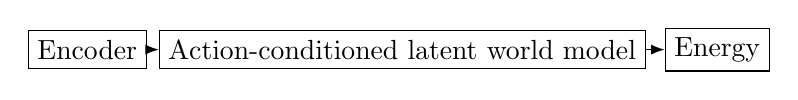
\begin{tikzpicture}[>=Latex]
		\node[draw] (encoder) at (0,0) {Encoder};
		\node[draw, align=center] (world_model) at (4,0) {Action-conditioned latent world model};
		\node[draw] (energy) at (8,0) {Energy};
		\draw[->] (encoder) -- (world_model);
		\draw[->] (world_model) -- (energy);
	\end{tikzpicture}
\end{figure}

The encoder and world model are learnable; the energy can be learnable or non-learnable:
\begin{itemize}
	\item The encoder predicts a hidden representation from an image.\footnote{The goal is to eliminate any detail unnecessary for prediction}.
	\item The world model predicts the next hidden representation from a hidden representation, action, and latent representation.
	\item The energy predicts a scalar cost measuring how ``good'' a hidden representation is.
\end{itemize}
Like how young animals in an environment might first internally learn representations (by passive observation of environmental evolution) before dynamics (by active environmental interaction), learning could occur in stages:
\begin{enumerate}
	\item The encoder could be trained alone.
	\item The encoder could be trained together with the world model.
	\item The encoder and world model could be trained together with the energy.
\end{enumerate}
\end{frame}

\begin{frame}{Architecture (for rigour)}
Let $\mathrm{R}\in\N_{\geq 1}$ be a hidden space dimensionality,
and $\mathrm{Z}\in\N_{\geq 1}$ be a latent space dimensionality,
and $\mathcal{R}=\R^{\mathrm{R}}$ be a hidden space,
and $\mathcal{Z}=\R^{\mathrm{Z}}$ be a latent space,
and $\mathbb{P}_{\mathcal{Z}}$ be a probability measure on $\mathcal{Z}$.
\begin{align*}
	\phi
	&:
	\mathcal{X}\to\mathcal{R}
	\tag{encoder}
	\\
	\mathscr{F}
	&:
	\mathcal{R}\times\mathcal{A}\times\mathcal{Z}
	\to
	\mathcal{R}
	\tag{world model}
	\\
	\mathscr{C},\mathscr{V}
	&:
	\mathcal{R}\to\R_{\geq 0}
	\tag{energy}
\end{align*}
We can train $\mathscr{V}$ on $\sum_{i=t}^{\tau-1}\gamma^{i-t}c_{i}$ and $\mathscr{C}$ on $c_{t}$.

The solution can be given by a discounted sum planner like
\begin{align*}
	\mathcal{U}\mleft(
		\arg\min_{\bm{a}\in\mathcal{A}^{T}}
		\E_{\bm{z}\sim\mathbb{P}_{\mathcal{Z}}^{\otimes T}}\mleft[
			\sum_{t=1}^{T}
			\gamma^{t-1}
			\mathscr{C}\mleft(
				\mleft(
					\bigcirc_{i=1}^{t}
					\mathscr{F}\mleft(\cdot,a_{i},z_{i}\mright)
				\mright)(
					\phi(x)
				)
			\mright)
		\mright]
	\mright)
\end{align*}
where $x\in\mathcal{X}$ is an image,
and $\gamma\in\R_{[0,1]}$ is a discount factor,
and $T\in\N_{\geq 1}$ is a planning horizon.
\end{frame}

\begin{frame}{Appendix}
Let $n\geq 1$, and $X$ be a set, and $f_{1},\dots,f_{n}:X\to X$.
$$
	\bigcirc_{i=1}^{n}f_{i}
	=
	f_{n}\circ\dots\circ f_{1}
$$
\end{frame}

\end{document}
